\documentclass{bmd2023a}

\pagenumbering{roman}

\usepackage{caption}
\usepackage{subcaption}

\begin{document}

%% Titlepage variables

% Title
\title{Modeling and Implementation of a Reaction Wheel Stabilization System for
Low Speed Balance of a Cargo Bicycle}

% List authors for the title. Call \addauthor{name}{affiliationID} for every
% author. Authors will appear in the order off calls to \addauthor. Please
% manually specify the correct affiliation ID and an asterisk to the
% corresponding author
\addauthor{Jason K. Moore}{1,*}
\addauthor{Jeswin Koshy Cherian}{1}
\addauthor{Bj{\"o}rn Andersson}{2}
\addauthor{Oliver Lee}{2}
\addauthor{Anders Ranheim}{2}

% List authors with only initials for given names, displays only in footer.
\authorfooter{Moore, J. K., Cherian, J. K., Andersson, B. C., Lee, O., \&
  Ranheim, A.}

% List affiliations. Call \addaffiliation{id}{name}{EmailOrcidString} once for
% every distinct institution, where id specifies the affiliation ID (ensure
% that this corresponds to the IDs used with \addauthor), name specifies the
% affiliation name, and EmailOrcidString is a string listing emails and ORCIDs
% (optional) affiliated with this affiliation separating mail and ORCID using a
% comma and different author credentials using a semicolon.

\addaffiliation{1}{
  Delft University of Technology, The Netherlands
}{
  j.koshycherian@student.tudelft.nl;
  j.kmoore@tudelft.nl, ORCID 0000-0002-8698-6143
}
\addaffiliation{2}{
  ictech, Sweden
}{
  bjorn.andersson@ictech.se, ORCID 2222-2222-2222-2222;
  oliver.lee@ictech.se, ORCID 2222-2222-2222-2222;
  anders.ranheim@ictech.se, ORCID 3333-3333-3333-3333
}

% The following variables will be updated by the publisher, do not edit.
\doi{XX.XXXX/XX.XXXX}
\year{2023}
\editor{Firstname Lastname}
\submitteddate{dd/mm/yyyy}
\accepteddate{dd/mm/yyyy}
\publisheddate{dd/mm/yyyy}
\citation{}
\issn{2667-2812}
% End publisher variables.

%% End titlepage variables

\maketitle

\section*{Abstract:}

Cargo bicycle use has grown over the last decade with electrification
contributing to a rapid growth in the recent years.
With the growth of safer bicycle infrastructure in many countries, these
vehicles can be a greener, more energy efficient replacement for cars for a
variety of short and medium distance activities, e.g. "last mile" delivery or
transportation for families.
One particular problem cargo two-wheelers face is that the vehicles are hard to
balance and handle at low and near zero speeds. Delivery people need to quickly
park their vehicle without the need for a bicycle storage rack or cumbersome
kickstands for quick door calls. Similarly, parents need to seat and remove
their children from the vehicle without worrying that it would fall. Also,
both vehicles come to a stop in traffic many times throughout a trip. At every
instance near zero speed, balance assistance would simplify vehicle operation
for the rider; even enabling it as a new transportation mode for those with
limited motor skills and coordination.
Our goal for this work was to develop and test the feasibility of robotically
stabilizing a single track cargo bicycle at zero and near zero forward speeds.

\begin{figure}
  \centering
  \begin{subfigure}{0.45\textwidth}
    \centering
    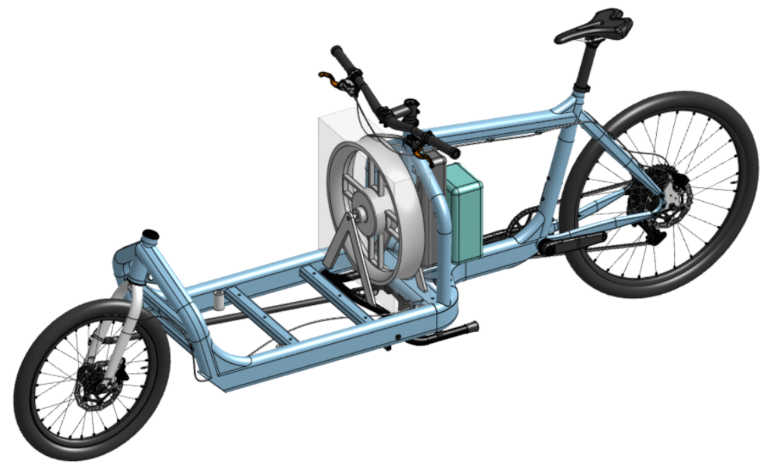
\includegraphics[height=4cm]{cad-model.png}
    \caption{CAD rendering of the envisioned reaction wheel on a common
      delivery bicycle model.}
    \label{fig:cad-model}
  \end{subfigure}
  \hfill
  \begin{subfigure}{0.45\textwidth}
    \centering
    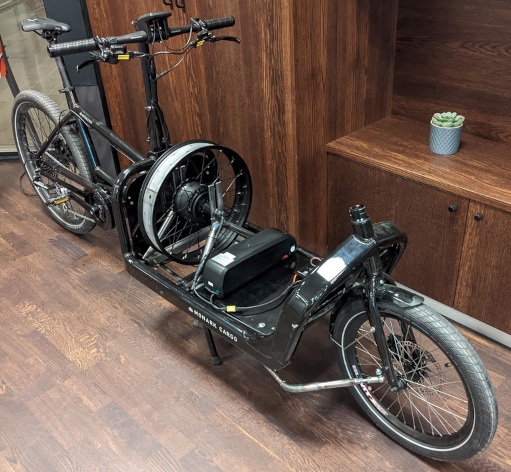
\includegraphics[height=4cm]{bike-photo.png}
    \caption{Prototype vehicle with a Bafung 48~\si{\volt} 1000~\si{\watt}
      motor with added rim mass to maximize the rotational inertia.}
    \label{fig:bike-photo}
  \end{subfigure}
\end{figure}

There is a long history of efforts to robotically stabilize single track
vehicles beginning with Brennan's monorail in the early
1900's~\citep{Barr1907}, to the motorcycle steer controller of
\citep{Ruijs1985}, and a too long list of models and demonstration of steer
control, control moment gryoscopes, reaction wheels, inverted pendulums and the
like. None of these solutions have become commercially viable, so our approach
tries to focus on the narrow need of near zero speed stabilization. We chose a
reaction wheel due to the low cost (<\$500), ability to stabilize roll at any
speed, and the possibility to fit the reaction wheel in a concealed manner in a
small portion of the cargo space.

To that end, we have developed a compact reaction wheel that fits in the cargo
space of a standard cargo bicycle. The reaction wheel is capable of applying
roll torques up to 200~\si{\newton\meter} to the vehicle, see
Figure~\ref{fig:cad-model}. This can stabilize the roll degree of freedom at
zero speed for roll angles up to about 10~\si{\degree}.

Figure~\ref{fig:initial-value-simulation} shows that the reaction wheel can
stabilize the vehicle from a 2~\si{\degree} disturbance within a second using
about 200~\si{\joule} and 100~\si{\newton\meter} of peak torque. A modern
e-bike battery can have 4M joules of energy available for use, so minimizing the
energy consumption from the reaction wheel while maximizing stability will need
to be investigated.

\begin{figure}
  \centering
  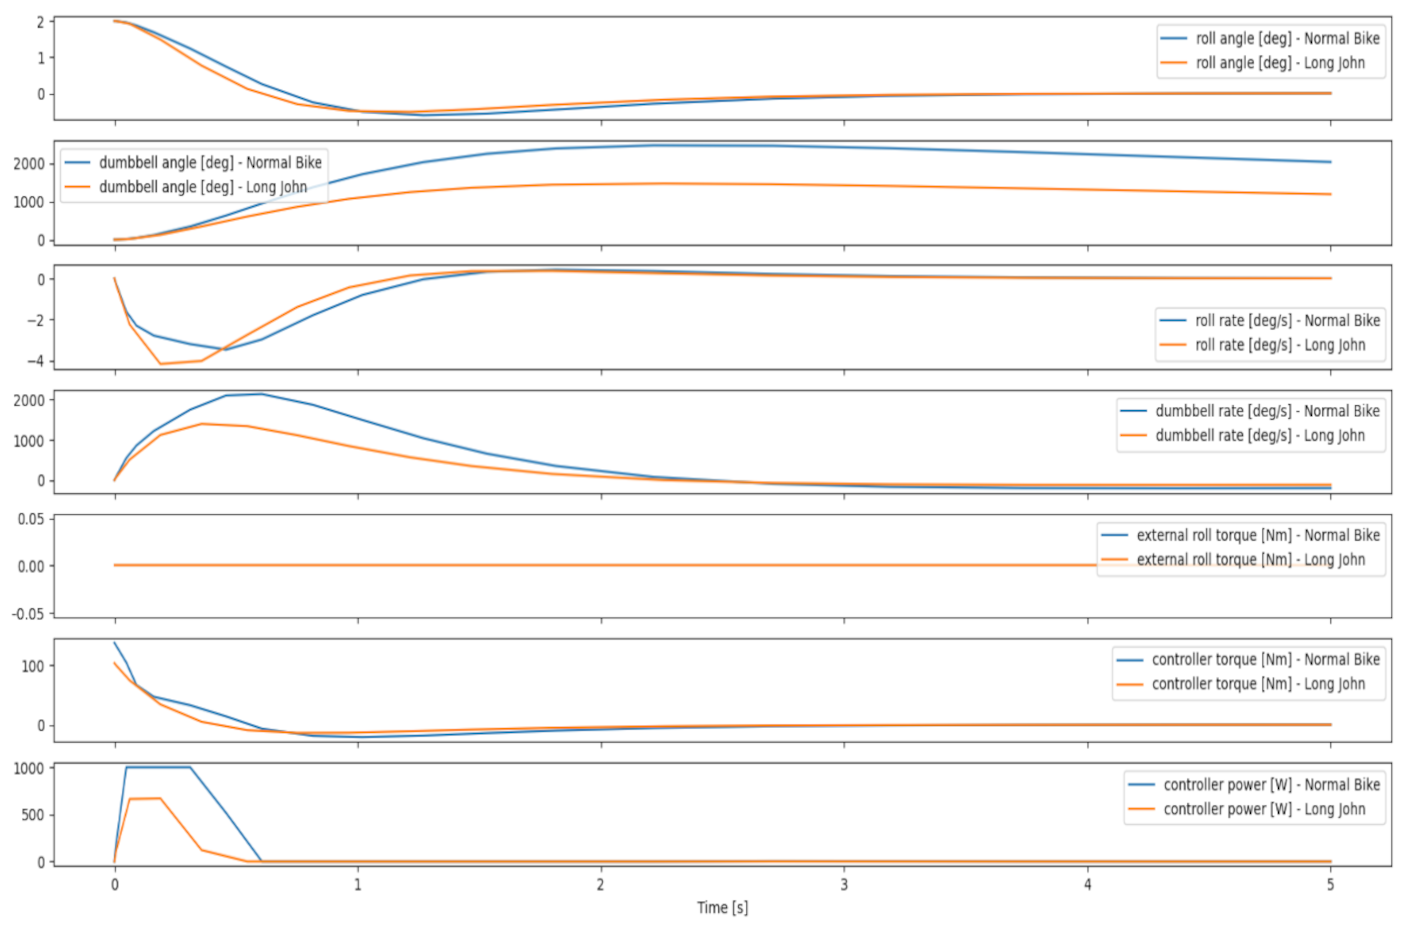
\includegraphics[width=12cm]{initial-value-simulation.png}
  \caption{Roll stabilization results at zero speed from an initial roll angle
    of 2~\si{\degree}}
  \label{fig:initial-value-simulation}
\end{figure}

The reaction wheel has some disadvantages, including significantly increasing
the mass of the vehicle (10 kg) as well as increasing the complexity and cost.
The energy consumption can be large when the system is constantly managing large
repeated disturbances, reducing the available range of an e-bike (possibly
drastically and unexpectedly to the rider). The reaction wheel will generate
pitching torques during rapid changes in heading (although we expect this to be
negligible). We will report on the validation and performance of the prototype
vehicle shown in Figure~\ref{fig:bike-photo} in the conference paper.

\bibliographystyle{apalike}
\bibliography{references.bib}

\end{document}
